\documentclass{standalone}
\usepackage{tikz}

\begin{document}
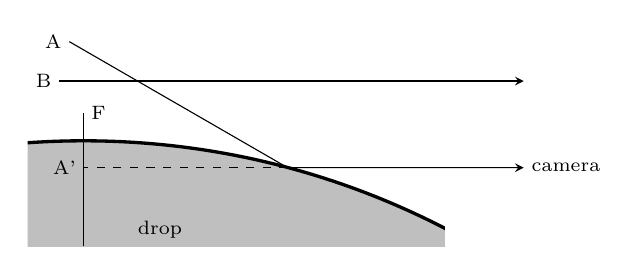
\begin{tikzpicture}
  \scriptsize % affects text nodes in this picture
  \newcommand{\dphi}{15} \newcommand{\rad}{10} \coordinate
  (dropcenter) at (-90-\dphi:\rad) ;
  % light rays
  \draw[->,>=stealth] (180-2*\dphi:3.2) node[left] {A} -- (0,0) --
  (3,0) node[right] {camera} ; \draw[->,>=stealth] (-2.9,1.1)
  node[left] {B} -- (3,1.1) ;
  % drop
  \clip (-3.3,1) rectangle (2,-1) ; \fill[gray!50,draw=black,very
  thick] (dropcenter) circle [radius=\rad] ; \node[above right] at
  (-2,-1) {drop} ;
  % virtual light ray
  \draw[dashed] (0,0) -- (0,0 -| dropcenter) node[left] {A'} ;
  % focal plane
  \draw[very thin] (dropcenter |- 0,-1) -- +(0,1.7) node[right] {F} ;
\end{tikzpicture}
\end{document}
